
%% bare_conf.tex
%% V1.4b
%% 2015/08/26
%% by Michael Shell
%% See:
%% http://www.michaelshell.org/
%% for current contact information.
%%
%% This is a skeleton file demonstrating the use of IEEEtran.cls
%% (requires IEEEtran.cls version 1.8b or later) with an IEEE
%% conference paper.
%%
%% Support sites:
%% http://www.michaelshell.org/tex/ieeetran/
%% http://www.ctan.org/pkg/ieeetran
%% and
%% http://www.ieee.org/

%%*************************************************************************
%% Legal Notice:
%% This code is offered as-is without any warranty either expressed or
%% implied; without even the implied warranty of MERCHANTABILITY or
%% FITNESS FOR A PARTICULAR PURPOSE!
%% User assumes all risk.
%% In no event shall the IEEE or any contributor to this code be liable for
%% any damages or losses, including, but not limited to, incidental,
%% consequential, or any other damages, resulting from the use or misuse
%% of any information contained here.
%%
%% All comments are the opinions of their respective authors and are not
%% necessarily endorsed by the IEEE.
%%
%% This work is distributed under the LaTeX Project Public License (LPPL)
%% ( http://www.latex-project.org/ ) version 1.3, and may be freely used,
%% distributed and modified. A copy of the LPPL, version 1.3, is included
%% in the base LaTeX documentation of all distributions of LaTeX released
%% 2003/12/01 or later.
%% Retain all contribution notices and credits.
%% ** Modified files should be clearly indicated as such, including  **
%% ** renaming them and changing author support contact information. **
%%************************************************uppfylla*************************


% *** Authors should verify (and, if needed, correct) their LaTeX system  ***
% *** with the testflow diagnostic prior to trusting their LaTeX platform ***
% *** with production work. The IEEE's font choices and paper sizes can   ***
% *** trigger bugs that do not appear when using other class files.       ***                          ***
% The testflow support page is at:
% http://www.michaelshell.org/tex/testflow/



\documentclass[conference]{IEEEtran}
% Some Computer Society conferences also require the compsoc mode option,
% but others use the standard conference format.
%
% If IEEEtran.cls has not been installed into the LaTeX system files,
% manually specify the path to it like:
% \documentclass[conference]{../sty/IEEEtran}
\usepackage[utf8]{inputenc}
\usepackage[swedish]{babel}
\usepackage[pdftex]{graphicx}
\usepackage[pdfborder={0 0 0}]{hyperref}
\graphicspath{{Images/}}
\DeclareGraphicsExtensions{.pdf,.png,.jpg}
% correct bad hyphenation here
\hyphenation{op-tical net-works semi-conduc-tor}

\begin{document}
%
% paper title
% Titles are generally capitalized except for words such as a, an, and, as,
% at, but, by, for, in, nor, of, on, or, the, to and up, which are usually
% not capitalized unless they are the first or last word of the title.
% Linebreaks \\ can be used within to get better formatting as desired.
% Do not put math or special symbols in the title.
\title{Vad är en bra projektmetod för små IT-projekt?}


% author names and affiliations
% use a multiple column layout for up to three different
% affiliations
\author
    {
      \IEEEauthorblockN{Sebastian Heimlén\textsuperscript{1},
        Henrik Björklund\textsuperscript{2},
        Yobart Amino\textsuperscript{3},
        Teo Klestrup Röijezon\textsuperscript{4}}
        \IEEEauthorblockA{\textit{KTH Royal Institute of Technology}
          \textit{Isafjordsgatan 22, 164 40 Kista, Sweden}\\
          \texttt{\textsuperscript{1}heimlen@kth.se}\\
          \texttt{\textsuperscript{2}hebjo@kth.se}\\
          \texttt{\textsuperscript{3}yobart@kth.se}\\
          \texttt{\textsuperscript{4}teo@nullable.se, roijezon@kth.se}
         }
    }

% make the title area
\maketitle

% As a general rule, do not put math, special symbols or citations
% in the abstract
\begin{abstract}
  this is an abstract.

  \textbf{\textit{keywords} - with keywords}
\end{abstract}

\IEEEpeerreviewmaketitle

\section{Om detta dokument och undersökning}
Detta dokument är ett försök att på ett vetenskapligt sätt undersöka projektmetoder inom små IT-projekt. Dokumentet är också delvis en träning på att skriva vetenskapliga rapporter och en övning inför examensarbetet. Dokumentet riktar sig mot akademin och specifikt mot kursens examinator som kommer att utvärdera rapporten enligt ''Blooms taxonomi'' \cite{krathwohl10}.\\
\\
Rapportens disposition är som följer. Sektion \ref{sec:intro} introducerar rapporten. Sektion \ref{sec:teori} redovisar bakomliggande teori och ingenjörspraxis. Sektion \ref{sec:under} redovisar vår undersökningsmetod. Sektion \ref{sec:genom} beskriver genomförandet. Sektion \ref{sec:res} redovisar resultatet av undersökningen. I sektion \ref{sec:analys} analyseras undersökningen och eventuella förbättringsförslag lämnas. I sektion \ref{sec:disk} diskuteras undersökningen och resultatet av undersökningen. Sektion \ref{sec:slutord} innehåller slutord. \\
\\
Detta dokuments trovärdighet anses vara hög, då undersökningsmetoden som använts är förankrad i Anderssons och Ekholms rapport som avhandlar vetenskaplighet i IT-projekt \cite{Andersson02}, vilket i sin tur leder till att resultaten är framtagna på ett vetenskapligt sätt. De projektmetoder vi undersöker är erkända och välanvanda inom IT-projekt, och dokumentet refererar till erkända böcker, tidsskrifter samt vetenskapliga texter. Dessa egenskaper bygger tillsammans upp projektets trovärdighet och vi är övertygade om att en likadan undersökning med lika många deltagare och samma förutsättningar skulle komma fram till så gott som samma slutsatser som vi har gjort.

\section{Introduktion} \label{sec:intro}

\subsection{Bakgrund}
Detta dokument är en del av examinationen i kursen ''Projekt och projektmetoder'' i vilket studenter i små grupper genomför ett IT-projekt som innefattar både hårdvara, mjukvara, datornätverk samt elektronik. Syftet med att genomföra projektet är att undersöka samt analysera olika projektmetoder, dessa analyser ska sedan diskuteras och framföras i denna rapport för att kunna besvara frågeställningen ''Vad är en bra projektmetod för små IT-projekt''.\\
\\
Kursens syfte är att fördjupa studenternas kunskap inom projektmetodik och skall fungera som en förberedelse inför både examensarbete samt det fortsatta arbetslivet efter examen. Kursen projektgrupper består av både data- samt elektrostudenter, och tanken bakom detta är att studenter från de olika programmen har olika expertisområden, vilket leder till att olika studenter har olika ansvarsområden inom projektgruppen, ett mål med kursen är att projektgruppen tillsammans ska utvecklas och dela med sig av sin kunskap, vilket leder till att samtliga medlemmar ytterliggare utvecklas på en personlig nivå.

\subsection{Problemformulering}
Den övergripande frågeställningen är som tidigare nämnt ''Vad är en bra projektmetod för små IT-projekt?''. För att besvara denna frågeställning måste gruppen först undersöka samt komma överens om vad en bra projektmetod är. En vettig utgångspunkt för att beskriva en bra projektmetod är projekt-triangeln \cite[s. 128-129]{Eklund14}. En bra projektmetod kan då beskrivas som en metod där projektgruppen på ett strukturerat och planerat vis tar fram en produkt som tillfredställer kundens krav och ej överskrider projektets budget. En bra projektmetod utvecklar också under arbetets gång projektgruppens effektivitet och sammarbetsförmåga. En bra projektmetod innefattar hjälpmedel som underlättar och förbättrar arbetsgången och tillåter projektgruppen att snabbt och ofta ändra arbetssätt, arbetsbörda och/eller förväntat resultatet av projektarbetet. Detta är grundkraven för en bra projektmetod och det är därför som agila och iterativa projektmetoder är så populära inom IT-projekt.\\
\\
Efter att ha sanktionerat denna definition av vad en bra projektmetod är blir det betydligt enklare och tydligare att resonera kring den övergripande frågeställningen.
\subsection{Undersökningsstrategi/lösningsstrategi}
Strategin för att undersöka och hitta svar till denna frågeställning har varit att genomföra en fallstudie i vilken projektgruppen genomfört ett litet IT-projekt. Inom detta projekt testas ett antal förvalda projektmetoder och varje medlem har tagit en specifik roll i projektet. Det är sedan varje medlems uppgift att inom denna roll experimentellt under projektets gång samla in information och intryck om vilka projektmetoder som fungerar bra och varför inom den specifika roll medlemmen besitter. Dessa intryck ska sedan analyseras och slutsatser skall dras, och det är dessa analyser och slutsatser som denna rapport avser avhandla.

\subsection{Relaterade arbeten}

\subsection{Avgränsningar}
Teorierna i denna rapport avgränsas genom att endast vissa förvalda projektmetoder tas upp, samt relativa teorier om dessa metoder. Dessa teorier begränsas till stor del av givna artiklar och dokument med viss komplimenterande dokument. Utöver detta så avgränsas också teorierna då projektet genomförs i en studiemiljö i grupper av studenter och samtliga grupper utför samma projektuppdrag.

\section{Teori och ingenjörspraxis} \label{sec:teori}
Detta kapitel listar och i viss mån beskriver teorier och ingenjörspraxis som använts i undersökningen. Det finns två underkapitel, Litteraturstudie och Förstudie.
\subsection{Litteraturstudie}
I genomförandet av denna fallstudie har flera källor konsulterats, och i detta kapitel anges dessa källor. Förutom de källor som anges finns förmodligen andra, och möjligtvis bättre, källor som ej konsulterats.\\

\noindent \textbf{Övergripande källor för hela projektet}
\begin{itemize}
\item Boken \textit{Software Engineering} av Ian Sommerville \cite{Sommerville10}.
\\
\item Handboken \textit{Scrum and XP from the Trenches} av Henrik Kniberg \cite{Kniberg07}.
\\
\item Handboken \textit{KanBan och Scrum, få det bästa av två världar} av Henrik Kniberg och Mattias Skarin \cite{Kniberg10}.
\\
\item Artikeln \textit{Industrial Scale Agile, from Craft to Engineering} av Ivar Jacobson, Ian Spence och Ed Seidewitz \cite{Jacobson16}.
\\
\end{itemize}

\noindent \textbf{Kundrepresentant}
\begin{itemize}
\item lista av källor
\\
\end{itemize}

\noindent \textbf{Analytiker}
\begin{itemize}
\item lista av källor
\\
\end{itemize}

\noindent \textbf{Utvecklare}\\
\indent Denna roll existerar i projektet, men det har ej varit en del av undersökningen och vi utelämnar därför rollen ur rapporten.\\
\\
\noindent \textbf{Testare}
\begin{itemize}
\item lista av källor
\\
\end{itemize}

\noindent \textbf{Ledning och styrning (Sebastian Heimlén)}
\begin{itemize}
\item \textit{Software Engineering} av Ian Sommerville \cite[kap. 22,23,26]{Sommerville10}. Dessa kapitel behandlar projektmetodik.
\\
\item Rapporten \textit{Vetenskaplighet - Utvärdering av tre implementeringsprojekt inom IT Bygg och Fastighet 2002} skriven av Niclas Andersson och Anders Ekholm \cite{Andersson02}.
\\
\item Boken \textit{Arbeta i projekt - individen, gruppen, ledaren} av Sven Eklund \cite{Eklund14}.
\\
\end{itemize}

\subsection{Förstudie}
Enligt undersökningsstrategin så skall någon projektmetod prövas i ett praktiskt projekt och utifrån de erfarenheter som fås görs en värdering av använda metoder. Frågan är då vilken ansats av projektmetod som skall användas. Eftersom erfarenheten av projektarbete hos studenterna i denna kurs är liten så fanns det ett färdigt förslag till ansats av projektmetod. Tidigare kursomgångar och lärarens förslag har mynnat ut i följande ansats. Projektmetoden framgår med god tydlighet av de arbetstavlor som definierats i ansatsen, se figur \ref{forslagsprintbacklog} och \ref{forslagproductbacklog}. Då litteraturstudie och kursteori i form av föreläsningar skett löpande under kursen så har projektgruppens egna förstudie gjort likaså. Detta har lett till att den föreslagna ansatsen iterativt förändrats och formats allt eftersom projektgruppens undersökning fortskridit.
Resultatet av förstudien är att metoderna, som anges i följande kapitel, har valts för undersökningens genomförande.
\subsubsection{Anslagstavla}

\begin{figure}[!ht]
\centering
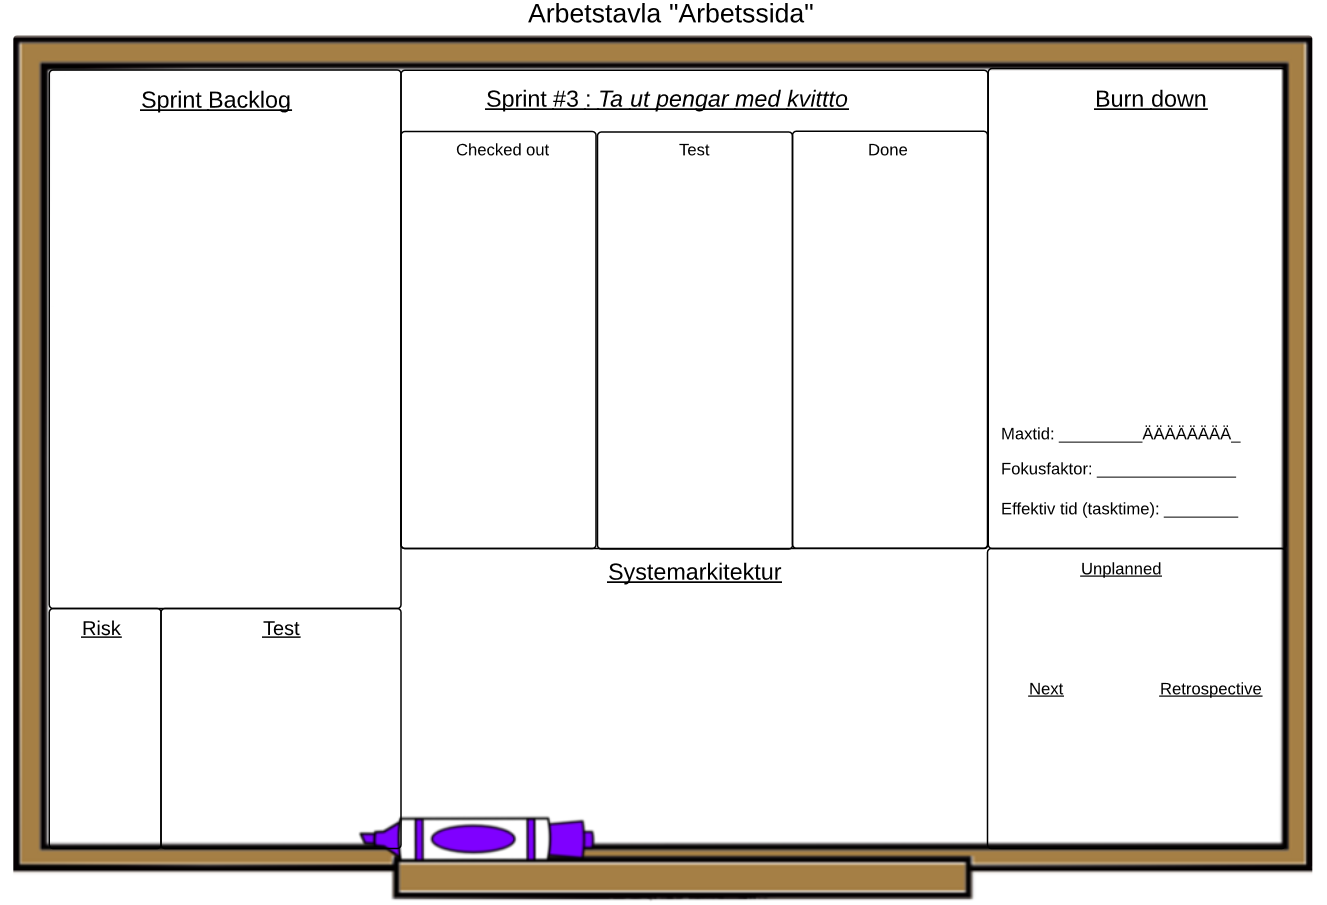
\includegraphics[width=3in]{forslagsprintbacklog}
% where an .eps filename suffix will be assumed under latex,
% and a .pdf suffix will be assumed for pdflatex; or what has been declared
\DeclareGraphicsExtensions.
\caption{Föreslaget Exempel på en intern sida för projektgruppen.}
\label{forslagsprintbacklog}
\end{figure}

\begin{figure}[!ht]
\centering
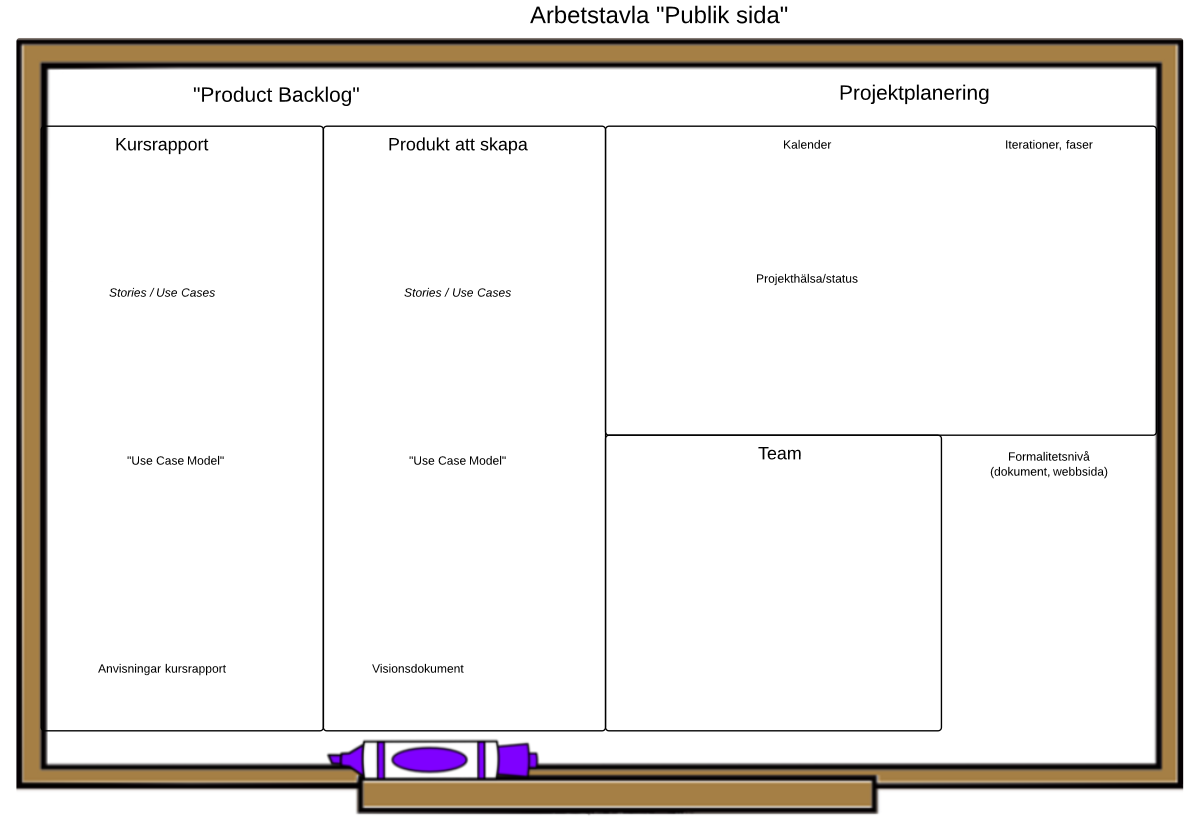
\includegraphics[width=3in]{forslagproductbacklog}
% where an .eps filename suffix will be assumed under latex,
% and a .pdf suffix will be assumed for pdflatex; or what has been declared
\DeclareGraphicsExtensions.
\caption{Föreslaget Exempel på en public sida för projektgruppen.}
\label{forslagproductbacklog}
\end{figure}

\subsubsection{Scruminspirerade projektaktiviteter (vald ansats)}



% use section* for acknowledgment
\section{Undersökningsmetoder} \label{sec:under}
Detta kapitel beskriver vilka metoder som använts i undersökningen. Metoderna är valda och specificerade så att de skall kunna ge svar på ett antal följdfrågor som identifierats i denna undersökning. Först anges frågorna och sedan följer metodbeskrivning.
\subsection{Frågor att besvara i undersökningen}

\subsection{Metodbeskrivning}

\textbf{Metod 1: Undersökningsmetod}

%Exempel på hur man lägger in en bild
\begin{figure}[!ht]
\centering
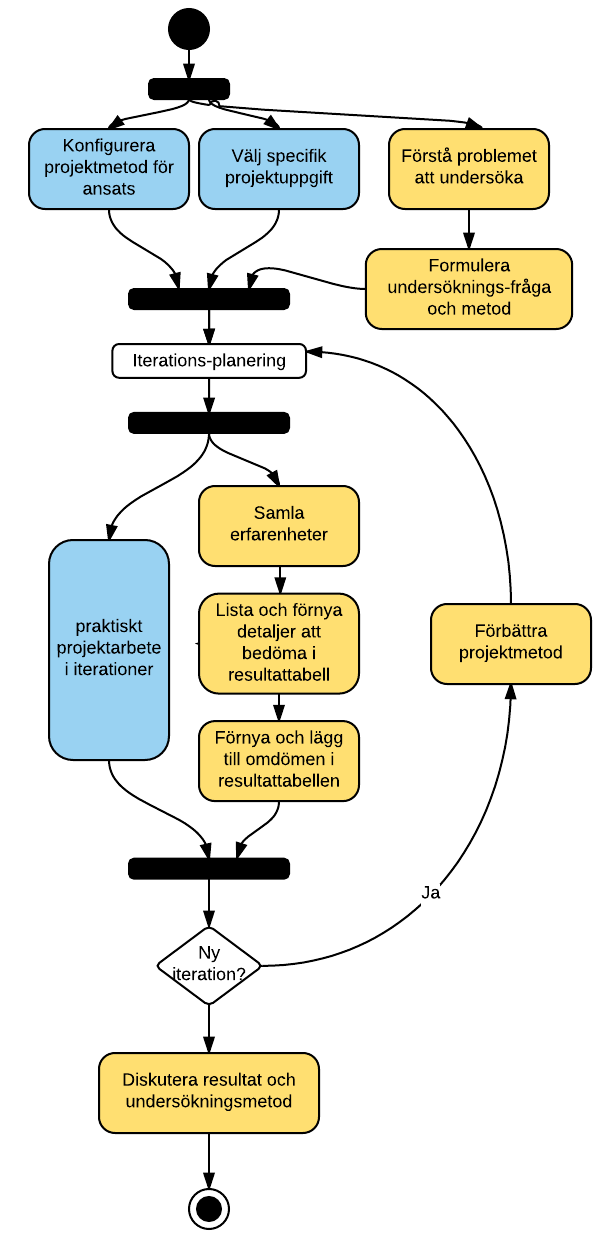
\includegraphics[width=2.5in]{invmethod}
% where an .eps filename suffix will be assumed under latex,
% and a .pdf suffix will be assumed for pdflatex; or what has been declared
\DeclareGraphicsExtensions.
\caption{Undersökningsmetod för ``Vad är en bra projektmetod för små IT-projekt?''.}
\label{undersokningsmetod}
\end{figure}

\textbf{Metod 2: Begrepp}\\
\\
Begrepp som används följer om möjligt OMGs standard Essence \cite{Jacobson13}.
Följande bilder listar illustrativt centrala begrepp. I denna artikel kommer de engelska begreppen att fritt översättas till svenska då risken för missförstånd anses liten.
\section{Genomförande} \label{sec:genom}
\textbf{NEDAN VISAS GENERELL LAYOUT FÖR DE ENSKILDA DELARNA, SKRIV SOM LÖPANDE TEXT}
\begin{enumerate}
\item Kort om rollen.
\item Vad som provats i rollen
\item Hur det som provades fungerade som metod för "små IT-projekt".
\item Alternativa metoder som kan fungera bättre eller kan provas i framtiden.
\item Lyft fram ett antal bitar från try, keep, skip som har med rollen att göra. Ta fram det bästa och tänk hur det relaterar till rollen och projktmetoder för små IT-projekt.
\item Ta upp allt speciellt bra/dåligt i rollen, verktyg (git), metoder, processer osv.
\item Återkoppla till litteratur och referera.
\end{enumerate}

\subsection{Projektledning}

\subsection{Kundrepresentant}

\section{Resultat} \label{sec:res}

% An example of a floating table. Note that, for IEEE style tables, the
% \caption command should come BEFORE the table and, given that table
% captions serve much like titles, are usually capitalized except for words
% such as a, an, and, as, at, but, by, for, in, nor, of, on, or, the, to
% and up, which are usually not capitalized unless they are the first or
% last word of the caption. Table text will default to \footnotesize as
% the IEEE normally uses this smaller font for tables.
% The \label must come after \caption as always.
%
%\begin{table}[!t]
%% increase table row spacing, adjust to taste
%\renewcommand{\arraystretch}{1.3}
% if using array.sty, it might be a good idea to tweak the value of
% \extrarowheight as needed to properly center the text within the cells
%\caption{An Example of a Table}
%\label{table_example}
%\centering
%% Some packages, such as MDW tools, offer better commands for making tables
%% than the plain LaTeX2e tabular which is used here.
%\begin{tabular}{|c||c|}
%\hline
%One & Two\\
%\hline
%Three & Four\\
%\hline
%\end{tabular}
%\end{table}
\section{Analys / Förbättringsförslag} \label{sec:analys}

\section{Diskussion} \label{sec:disk}

\subsection{Metoddiskussion}

\subsection{Resultatdiskussion}

\subsection{Bidrag till vetenskaplighet, ingenjörserfarenhet (studenterfarenhet?)}

\section{Slutord} \label{sec:slutord}

% trigger a \newpage just before the given reference
% number - used to balance the columns on the last page
% adjust value as needed - may need to be readjusted if
% the document is modified later
%\IEEEtriggeratref{8}
% The "triggered" command can be changed if desired:
%\IEEEtriggercmd{\enlargethispage{-5in}}

% references section

% can use a bibliography generated by BibTeX as a .bbl file
% BibTeX documentation can be easily obtained at:
% http://mirror.ctan.org/biblio/bibtex/contrib/doc/
% The IEEEtran BibTeX style support page is at:
% http://www.michaelshell.org/tex/ieeetran/bibtex/
%\bibliographystyle{IEEEtran}
% argument is your BibTeX string definitions and bibliography database(s)
%\bibliography{IEEEabrv,../bib/paper}
%
% <OR> manually copy in the resultant .bbl file
% set second argument of \begin to the number of references
% (used to reserve space for the reference number labels box)
%\begin{thebibliography}{1}

%\bibitem{IEEEhowto:kopka}
%H.~Kopka and P.~W. Daly, \emph{A Guide to \LaTeX}, 3rd~ed.\hskip 1em plus
%  0.5em minus 0.4em\relax Harlow, England: Addison-Wesley, 1999.

%\bibitem{}

%\end{thebibliography}

\nocite{*}
\bibliographystyle{IEEEtran}
\bibliography{sources}

% that's all folks
\end{document}
